%%%%%%%%%%%%%%%%%%%%%%%%%%%%%%%%%%%%%%%%%%%%%%%%%%%%%%%%%%%%%%%%%%%%%%%%%%%%%%%%
%%%%%%%%%%%%%%%%%%   Vorlage für eine Abschlussarbeit   %%%%%%%%%%%%%%%%%%%%%%%%
%%%%%%%%%%%%%%%%%%%%%%%%%%%%%%%%%%%%%%%%%%%%%%%%%%%%%%%%%%%%%%%%%%%%%%%%%%%%%%%%

% Erstellt von Maximilian Nöthe, <maximilian.noethe@tu-dortmund.de>
% ausgelegt für lualatex und Biblatex mit biber

% Kompilieren mit
% latexmk --lualatex --output-directory=build thesis.tex
% oder einfach mit:
% make

\documentclass[
  tucolor,       % remove for less green,
  BCOR=12mm,     % 12mm binding corrections, adjust to fit your binding
  parskip=half,  % new paragraphs start with half line vertical space
  open=any,      % chapters start on both odd and even pages
  cleardoublepage=plain,  % no header/footer on blank pages
]{tudothesis}


% Warning, if another latex run is needed
\usepackage[aux]{rerunfilecheck}

% just list chapters and sections in the toc, not subsections or smaller
\setcounter{tocdepth}{1}

%------------------------------------------------------------------------------
%------------------------------ Fonts, Unicode, Language ----------------------
%------------------------------------------------------------------------------
\usepackage{fontspec}
\defaultfontfeatures{Ligatures=TeX}  % -- becomes en-dash etc.

% load english (for abstract) and ngerman language
% the main language has to come last
\usepackage[american, british]{babel}

% intelligent quotation marks, language and nesting sensitive
\usepackage[autostyle]{csquotes}

% microtypographical features, makes the text look nicer on the small scale
\usepackage{microtype}

%------------------------------------------------------------------------------
%------------------------ Math Packages and settings --------------------------
%------------------------------------------------------------------------------

\usepackage{amsmath}
\usepackage{amssymb}
\usepackage{mathtools}
\usepackage{braket}

% Enable Unicode-Math and follow the ISO-Standards for typesetting math
\usepackage[
  math-style=ISO,
  bold-style=ISO,
  sans-style=italic,
  nabla=upright,
  partial=upright,
  warnings-off={mathtools-colon,mathtools-overbracket}, % suppress some unnecessary warnings
]{unicode-math}
\setmathfont{Latin Modern Math}

% nice, small fracs for the text with \sfrac{}{}
\usepackage{xfrac}


%------------------------------------------------------------------------------
%---------------------------- Numbers and Units -------------------------------
%------------------------------------------------------------------------------

\usepackage[
  locale=DE,
  separate-uncertainty=true,
  per-mode=symbol-or-fraction,
]{siunitx}

%------------------------------------------------------------------------------
%-------------------------------- tables  -------------------------------------
%------------------------------------------------------------------------------

\usepackage{booktabs}       % \toprule, \midrule, \bottomrule, etc

%------------------------------------------------------------------------------
%-------------------------------- graphics -------------------------------------
%------------------------------------------------------------------------------

\usepackage{graphicx}
\usepackage{wrapfig}
% currently broken
% \usepackage{grffile}

% allow figures to be placed in the running text by default:
\usepackage{scrhack}
\usepackage{float}
\floatplacement{figure}{htbp}
\floatplacement{table}{htbp}

% keep figures and tables in the section
\usepackage[section, below]{placeins}

% allows to include PDFs as full pages
\usepackage{pdfpages}

% Set the PDF Version of this document to 1.7 (1.4 is the current default)
% This is needed so that PDFs with Version >1.5 can be included
\pdfvariable minorversion=7

%------------------------------------------------------------------------------
%---------------------- customize list environments ---------------------------
%------------------------------------------------------------------------------

\usepackage{enumitem}

%------------------------------------------------------------------------------
%------------------------------ Bibliographie ---------------------------------
%------------------------------------------------------------------------------

\usepackage[
  backend=biber,   % use modern biber backend
  sorting=none,
  autolang=hyphen, % load hyphenation rules for if language of bibentry is not
                   % german, has to be loaded with \setotherlanguages
                   % in the references.bib use langid={en} for english sources
]{biblatex}
\addbibresource{references.bib}  % the bib file to use
\DefineBibliographyStrings{german}{andothers = {{et\,al\adddot}}}  % replace u.a. with et al.


% Last packages, do not change order or insert new packages after these ones
\usepackage[pdfusetitle, unicode, linkbordercolor=tugreen, citebordercolor=tugreen]{hyperref}
\usepackage{bookmark}
\usepackage[shortcuts]{extdash}

%------------------------------------------------------------------------------
%-------------------------    Angaben zur Arbeit   ----------------------------
%------------------------------------------------------------------------------

\author{Joel Koch}
\title{Key Experiments in Particle Physics}
\date{29.02.2024}
\chair{Experimental Physics IV}
\division{Faculty Physics}
% \thesisclass{Bachelor of Science}
% \submissiondate{29. Februar 2024}

% tu logo on top of the titlepage
\titlehead{
\includegraphics[height=1.5cm]{logos/tu-logo-eng.pdf}}

\begin{document}
\frontmatter
\maketitle  % Auskommentiert, da der Titel "Arbeit zum Erlangen des akademischen Grades..." entfernt wurde

% \thispagestyle{plain}

\section*{Preface}

The summary of the course "Key Experiments of Particle Physics" from the winter semester of 2023/2024 will summarise one presentation from each session respectively.
It will be sorted not by the dates of the individual presentations but by the respective historical events.
The first chapter will be about semiconductors as they are used in the following experiments, except for the Wu experiment, and are thus a fundamental aspect of the detection of elementary particles.
The Wu experiment will be the second chapter being discussed, which provided the first experimental evidence for the violation of parity conservation in the weak interaction in 1956, leading to theoretical structures such as the $(V-A)$-structure and the CKM-Matrix and thus laying the foundation for particle physics.
The next chapter focuses on the discovery of the gluon in 1978, which took a significant step in the acceptance of the Standard Model of Particles (SM) \cite{Gaillard1998ui} as there had only been the photon discovered as one of the force-exchanging particles at the time \cite{DesyGluon}.
The last chapter will revise the oscillation of B-mesons ...
\tableofcontents

\mainmatter
% Hier beginnt der Inhalt mit Seite 1 in arabischen Ziffern
\chapter{The Wu Experiment}
\label{cha:wu_exp}

The Wu experiment focuses on the parity transformation $\hat P$, charge conjugation transformation $\hat C$ and its combination $\hat C\hat P$.
In physics, parity describes the symmetry of spatial coordinates.
A given point $(t, \vec x)$ would transform to $(t, -\vec x)$ under $\hat P$.
Classical physics is invariant under parity transformation and is thus conserving it.
The intrinsic parity of a particle is calculated via the spin $l$ by $ \hat P=(-1)^l$.
As classical physics is invariant under the change of sign in spatial coordinates, it is also invariant under the change of sign of electric charges.
In elementary particle physics, the change of sign of electric charges is called charge conjugation transformation $\hat C$ converting particles into anti-particles and vice versa, $\hat C \ket{e} = \ket{\bar e}$.
By 1957, significant discoveries of particles had already taken place, such as $e^\pm,\ \nu_e,\ \mu, p, \gamma,\ \pi$ and $K$.
Parity conservation was evident for the electromagnetic (EM), the strong and the gravitational interaction, but there was no experimental evidence for parity conservation in the weak interaction \cite{CaseStudies}.
For most physicists, it seemed self-evident that parity is conserved in the weak interaction as well.
In 1956 however, Tsung-Dao Lee (*1926) and Chen Ning Yang (*1922) considered the possibility that $\hat P$ can be violated in the weak interaction and proposed different experiments to test it  \cite{PhysRev.104.254}.
\begin{wrapfigure}{r}{5.5cm}
    \centering
    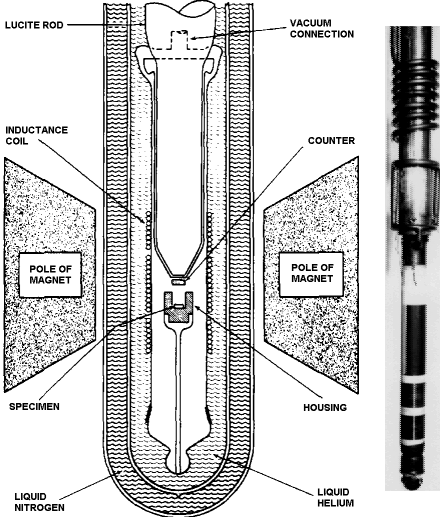
\includegraphics[width=0.35\textwidth]{figs/setup.png}
    \caption{Schematic illustration and photograph of the apparatus \cite{NIST}.}
    \label{fig:setup}
\end{wrapfigure}
The first to carry out such an experiment was Chien-Shiung Wu (1912-1997) when she was approached by Lee and Yang for her expertise in $\beta$-decay in 1956.
The experiment was based on the decay of Cobalt via $\cobalt\rightarrow \nickel+e^-+2\gamma+\bar\nu_e$.
Cobalt has a spin of 5 and was used because it decays via a $\beta$-decay into excited nickel with a spin of 4 meaning that the particles have to have the same spin direction.
Due to the polarization of the nucleus, the electrons are emitted either upwards or downwards.
The emission of the electrons is invariant under parity transformation if it is conserved in the weak interaction and vice versa.
A cerium magnesium nitrate (CMN)-crystal with a small layer of cobalt was used as the specimen and placed inside a housing necessary to hold the polarization \cite{CaseStudies} which was caused by a magnetic field.
A schematic illustration with a photograph of the used apparatus is shown in figure \ref{fig:setup}.
\begin{wrapfigure}{L}{5.5cm}
    \centering
    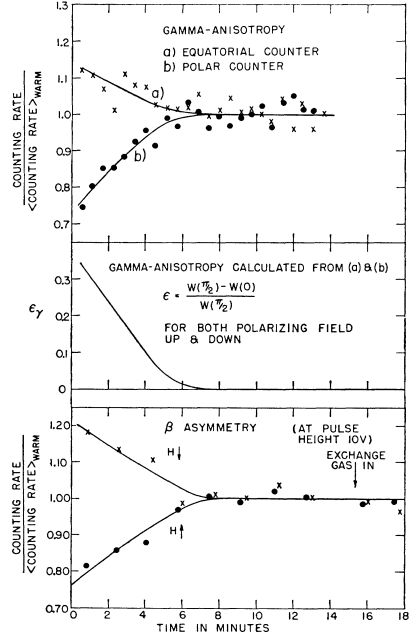
\includegraphics[width=0.4\textwidth]{figs/resultsWu.png}
    \caption{Measured results showing the gamma anisotropy and electron asymmetry for a polarizing magnetic field pointing up and down \cite{PhysRev.105.1413}.}
    \label{fig:resultsWu}
\end{wrapfigure}
An anthracene crystal was used as a scintillation counter and placed inside the lucite rod.
Sodium iodide gamma-scintillation counters were installed externally to measure the $\gamma$.
If the magnetic field is repolarized, the electron emission rates will stay the same if parity is conserved.
The $\gamma$-scintillation counters were used to measure the state of the polarization because the originally isotropic emission changes under parity transformation to an oval anisotropy as this is an EM process that conserves parity \cite{CaseStudies}.
The experimental results are shown in figure \ref{fig:resultsWu}.
The measured electron rates show a clear dependence on the polarization direction.
This asymmetry in the emission of electrons is violating parity conservation as the electrons prefer a direction in which to be emitted \cite{PhysRev.105.1413}.
By comparing the $\gamma$ and $\beta$ emissions for similarities, it can be seen that the $\beta$ asymmetry reduces when the $\gamma$ anisotropy reduces indicating that it is not due to misalignment of the apparatus.
Further systematic checks have been made showing no dependence on systematic uncertainties \cite{CaseStudies}.
Parity nonconservation in the weak interaction also implies the violation of charge conjugation assuming its combination is conserved.

The measured asymmetry was quantified by comparing the $\beta$ asymmetry with the $\gamma$ anisotropy. % which was difficult as it was difficult to measure the anisotropy.
But only a lower limit of $\alpha\leq -0.7$ could be measured because the anisotropy was difficult to measure.
Lee and Yang received a Nobel Prize while Wu did not.
A two-component neutrino theory published by Lee and Yang in 1957 introduces right-handed neutrinos and left-handed antineutrinos, both being massless and having a parity asymmetry of $\alpha=-1$ \cite{PhysRev.105.1671}.
Thus, a new experiment was designed to measure an asymmetry value of $\alpha=\num{-1.01(0.02)}$ \cite{CHIROVSKY1980127} which is in perfect agreement with the theory leading to the (V-A)-structure introduced by Richard Feynman and Murray Gell-Mann.
According to the Sakharov conditions from 1967¥ \cite{Gato-Rivera} the matter-antimatter asymmetry in the universe could be explained if, amongst other things, $\hat C$ and $\hat C\hat P$ can be violated which the Wu experiment demonstrated.
The search for $\hat C\hat P$-asymmetry is still researched today as the largest asymmetry yet was measured at LHCb in 2022 \cite{AntiSymmetryLHC}.
\chapter{The Discovery of the Gluon}

To organize hadrons in dependence on the quantum variables strangeness and isospin Murray Gell-Mann and Yuval Ne'eman proposed independently from each other the Eightfold Way in 1961.
Mesons with a spin parity configuration of $0^-$ and baryons with $\sfrac 12^+$ can both be organized in an octet while baryons with $\sfrac 32^+$ can be organized in a decuplet of which the tenth particle, the $\upOmega^-(sss)$ has been proposed theoretically before it has been found later \cite{Fritzsch2018}.
The early quark model was proposed by Gell-Mann and George Zweig in 1964 which consisted of only $u-,\ d-,\ s$-quark.
An electron-proton scattering event from 1968 revealed partons that took up half of the carried momentum and were thus the first indication of gluons \cite{Venker}.
A theoretical description is given by Quantum Chromodynamics (QCD) after which the baryon wave function must be antisymmetric thus leading to the introduction of colour as another quantum variable that can be either red, green or blue.
QCD is an $\text{SU}(3)$ gauge symmetry theory that describes the strong interaction predicting eight gluons as gauge bosons that can interact with themselves.
Particles with a colour charge can never be detected as a single particle, because the energy to separate two particles increases until a particle-antiparticle pair is produced, called confinement leading to quarks and gluons combining with other colour-carrying particles forming new hadrons.
These hadrons can in turn form new hadrons themselves building a cascade of particles called a jet which was first observed at the Stanford Positron Electron Asymmetric Rings (SPEAR) at $\SI{7.4}{\giga\eV}$ in 1975.
\begin{wrapfigure}{r}{5.5cm}
    \centering
    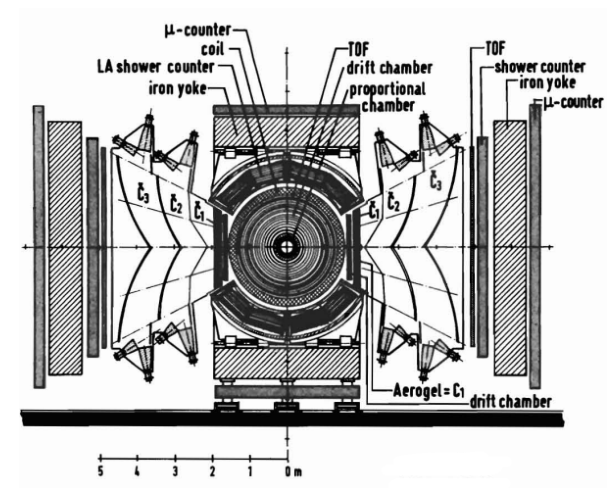
\includegraphics[width=0.4\textwidth]{figs/TASSO.png}
    \caption{Schematic image of the TASSO-detector \cite{TASSO:1979xej}.}
    \label{fig:TASSO}
\end{wrapfigure}
In the year 1979, all quarks except the top quark were found in experiments with the most recent discovery being the bottom quark in 1977 with no experimental evidence for gluons thus far.
Due to corrections at high energies, an electron-positron collision can produce a quark-antiquark pair with an additional gluon in a three-jet event as suggested by John Ellis.
The gluon emission can be seen as the equivalent of bremsstrahlung in QCD.
The transition between a two and a three-jet event is continuous as the jets get broader es the energy increases until they can split up into three distinct jets with one for each particle.
A two jet-event starts at energies of $\SI{7.4}{\giga\eV}$ and turns into a three-jet event at $\sim\SI{20}{\giga\eV}$.
The first gluon was discovered in a three-jet event at a center of mass energy of $\SI{27.4}{\giga\eV}$ with the Two Arm Spectrometer Solenoid detector (TASSO) at the Positron-Electron Tandem Ring Accelerator (PETRA) in 1979 which is part of the Deutsches Elektronen-Synchrotron (DESY).
A schematic picture of TASSO is shown in figure \ref{fig:TASSO}.
It started building in 1976 and was finished just two years later and had a ring accelerator with a circumference of $\SI{2.304}{\kilo\meter}$. %that could reach $\SI{27}{\giga\eV}$.
The detector had two hadron-identifying arms, one aerogel and two gas Cherenkov detectors and time-of-flight and shower counters.
Event shape variables were introduced as perturbation theory was not useable for low energies which could be used to distinguish between different QCD models, one in which there are no gluons and one in which there are.
The experimental results were in good agreement with the gluon model, as can be seen in figure \ref{fig:GluonResultsA} that shows predictions for different models \cite{Branson:1994eu}.
By measuring the angle in a Lorentz-boosted center-of-momentum frame, called the Ellis-Karliner angle, it is possible to analyse the spin of the gluon.
The Ellis-Karliner angle distribution from TASSO is shown in figure \ref{fig:GluonResultsB} in which the experimental data matches the theoretical prediction of a vector particle proving that the gluon has a spin of 1 \cite{Venker, Soding:1996zk}.
The discovery of the gluon is the perfect example of theory and experiments working together to discover new parts of physics as the gluon was originally predicted by QCD as a vector boson that could be emitted in three-jet events and was discovered in such an event with the exact characteristics it was predicted to have.

\begin{figure}
    \centering
    \begin{subfigure}[B]{.5\textwidth}   % 1st subfigure
        \centering
        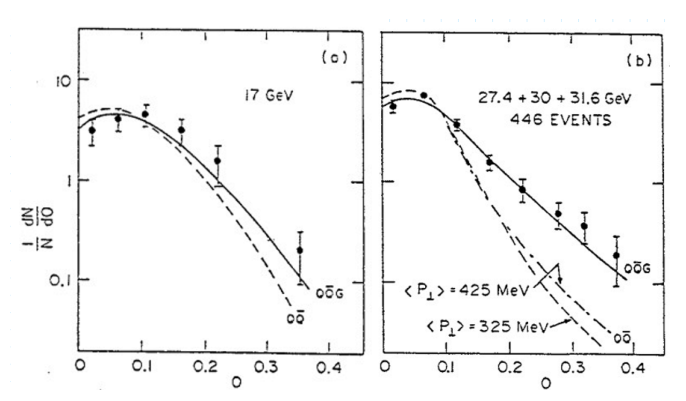
\includegraphics[width=1.1\textwidth]{figs/gluonResultsA.png}
        \caption{Experimental results comparing comparing different QCD models\cite{Branson:1994eu}.}
        \label{fig:GluonResultsA}
    \end{subfigure}
    \begin{subfigure}[B]{.45\textwidth}   % 2nd subfigure
        \centering
        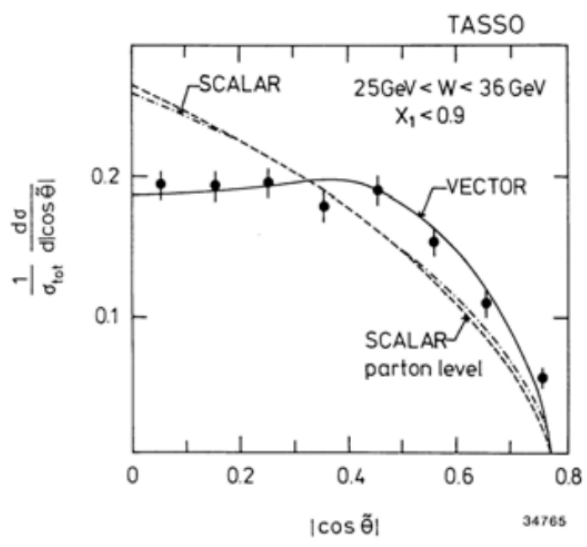
\includegraphics[width=.8\textwidth]{figs/gluonResultsB.png}
        \caption{Ellis-Karliner angle distribution from TASSO \cite{Soding:1996zk}.}
        \label{fig:GluonResultsB}
    \end{subfigure}
    \caption{Experimental results from the TASSO detector \cite{Branson:1994eu, Soding:1996zk}.}
    \label{fig:resultsGluonBoth}
\end{figure}

The strong coupling constant $\alpha_S$ which determines the strength of the interaction can be calculated by measuring the cross-section of three- versus two-jet events.
The compact muon solenoid experiment (CMS) at the large hadron collider (LHC) measured a value of $\alpha_S=\num{0.1448(0.0014)}$ at $\sqrt s=\SI{7}{\tera\eV}$ in 2011 \cite{CMS:2013vbb}.
\chapter{Semiconductor Detectors}\label{Semiconductors}

The earliest studies of semiconductor detectors date back to 1833 when Faraday discovered the temperature dependence of the conductivity of silver sulphide.
Nearly a hundred years later, Wilson described a band theory of solids in 1931, in which quantum mechanics explains the characteristics of semiconductors.
The electrical conductivity can be described by the valence band (VB) which consists of positively charged quasiparticles that are called holes $h^+$ and the conduction band (CB) which is filled with electrons \cite{KolanoskiWermes}.
The band theory of solids distinguishes three types of conductive solids.
Insulators with a band gap of $E_G\approx \SI{9}{\eV}$, semiconductors with $E_G\approx \SI{1}{\eV}$ and conductors with no gap.
The properties of semiconductors can be changed by inserting impurities into the crystal structure.
If an atom with five electrons, called a donor, is inserted into an element with four electrons, an excessive conduction electron appears.
If an atom with three electrons, called an acceptor, is inserted into an element with three electrons, an excessive hole appears.
Semiconductors doped with donors are called n-doped while those doped with acceptors are called p-doped.
When both types of doped semiconductors are combined they form a diode.
Drifting and combining of $e^-/h^+$ forms an electrical field at the junction of the semiconductor which is called the depletion zone.
If an external positive voltage at the p side relative to the n side is applied, this electrical field is weakened and current can flow which is called forward bias.
In reverse bias, the electrical field is strengthened and the depletion zone increases. 
This configuration is used in detectors to measure ionizing particles.
\begin{figure}[H]
    \centering
    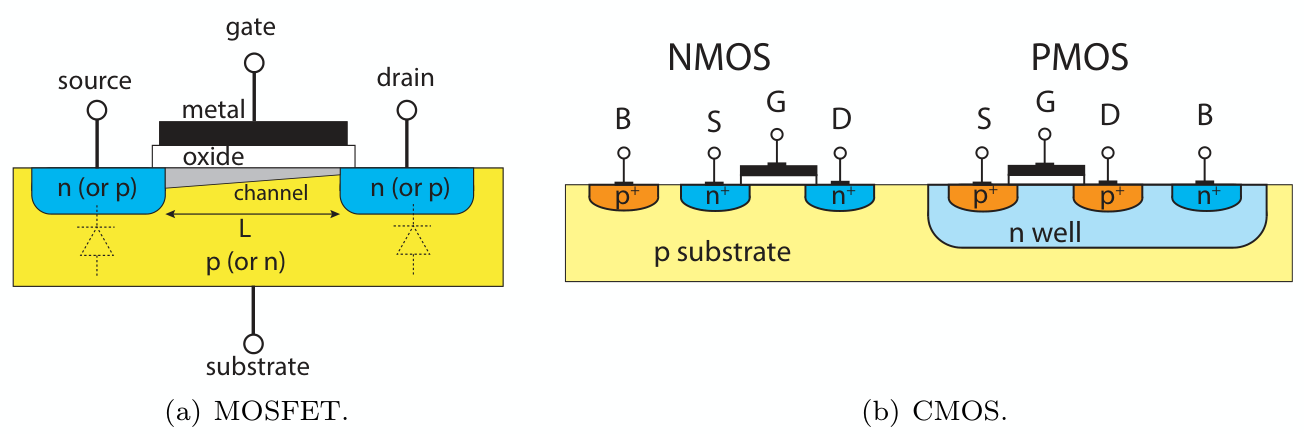
\includegraphics[width=0.69\textwidth]{figs/MOS.png}
    \caption{Schematic illustration of a MOSFET and a CMOS semiconductor \cite{KolanoskiWermes}.}
    \label{fig:MOStransition}
\end{figure}
The most used semiconductor detectors are complementary metal-oxide-semiconductors (CMOS) consisting of a part with a p-doped substrate and an n-doped drain terminal (NMOS) and a part with the reverse (PMOS).
Figure \ref{fig:MOStransition} shows a CMOS and a widely in field-effect transistor used semiconductor (MOSFET).

The simplest design of detectors is a pn area diode consisting of a $\SI{300}{\micro\meter}$ thick p and n-doped area.
An additional guard ring can reduce the electrical noise.
Dividing the area into strips or pixels ($\text{length}<\SI{100}{\micro\meter}$) yields one or even two spatial coordinates but increases the readout difficulty.
There are two different types to read out the information from the collection diodes.
Hybrid pixel sensors have the readout electronics on a different chip which is a laborious assembly and resides in a large material thickness, the sensor, however, can be separately optimized to the readout components.
Monolithic pixel sensors reduce their material by an entire order of magnitude but not all production lines are suited to produce such sensors.
As pixel detectors are used to reconstruct traces for example in the ATLAS Experiment due to their good resolution with an uncertainty of $\sigma_x=\sfrac{\text{pitch}}{\sqrt{12}}$ \cite{Tom}, they are placed closest to the collision vertex where a lot of charged particles pass through them causing damage to the detector substrate.
Such radiation damage can cause a change in effective doping concentration leading to deactivated donor or acceptor atoms.
They can furthermore cause trapping where $e^-/h^+$ are trapped in defects of the crystal structure and are released later.
These defects can form energy levels that excite $e^-/h^+$ easier and cause a flow in current.
Radiation damage can be reduced by cooling \cite{Tom}.
\begin{wrapfigure}{l}{7.5cm}
    \centering
    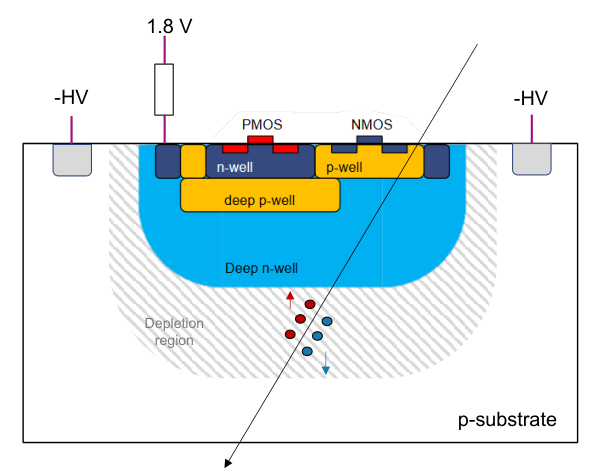
\includegraphics[width=0.5\textwidth]{figs/MightyPix.png}
    \caption{Schematic illustration of a MightyPix \cite{MightyPix}.}
    \label{fig:MightyPix}
\end{wrapfigure}
A track is reconstructed by forming groups of measurement points, called tracklets which require a good spatial and time resolution of the pixel detectors.
In each of the tracklets every possible combination is built but only those that point to the interacting point are accepted, forming a track when a series of tracklets match.
An application of pixel detectors is given in the example of MightyPix, a design sketch of possible pixel detectors used in the second upgrade of the LHC that is shown in figure \ref{fig:MightyPix}.
Their requirements for the upgrade include a time resolution of $<\SI{3}{\nano\second}$, and a pixel size of $~\SI{50}{\micro\meter}\times\SI{150}{\micro\meter}$.
Semiconductor detectors in the form of pixel detectors provide good time and space resolution which is why particle detectors are indispensable without them.
However, the implementation of pixel detectors brings new challenges like the power distribution or the cooling. %of the detectors.

\chapter{Oscillation of neutral $B$-mesons}

The phenomenon of neutral mesons transforming into their respective antiparticle was first investigated by Gell-Main and Pais in 1955 \cite{PhysRev.97.1387}.
The CKM-matrix was introduced as an extension of the Cabbibo matrix in 1973 after discovering $CP$ violation which could not be explained with 4-quark-mixing \cite{10.1143/PTP.49.652}.
Each element of the matrix describes a transition between quark generations.
The neutral B meson $B^0_d(d\bar b)$ or respectively $B^0_s(s\bar d)$ can oscillate via two components, the on-shell $(E^2= p^2+m^2)$ and off-shell $(E^2\neq p^2+m^2)$ components.
Both are shown in \ref{fig:feynmanOnshell} and \ref{fig:feynmanOffshell} respectively.
\begin{figure}
    \centering
    \begin{subfigure}[B]{.5\textwidth}   % 1st subfigure
        \centering
        \includegraphics[width=.8\textwidth]{figs/feynmanOnshell.png}
        \caption{On-shell contribution.}
        \label{fig:feynmanOnshell}
    \end{subfigure}
    \begin{subfigure}[B]{.45\textwidth}   % 2nd subfigure
        \centering
        \includegraphics[width=.8\textwidth]{figs/feynmanOffshell.png}
        \caption{Off-shell contribution.}
        \label{fig:feynmanOffshell}
    \end{subfigure}
    \caption{Feynman diagram showing the neutral B meson oscillation \cite{Kpopp}.}
    \label{fig:feynmanDiagram}
\end{figure}
Measuring the oscillation frequency yields precise measurements of $V_{q_u b}$ and $V_{q_u d/s}$.
A time evolution can be deduced by introducing a mixing matrix in which non-diagonal elements occur due to oscillations via the box diagram \ref{fig:feynmanOnshell} and the on-shell contributions.
By diagonalising the mixing matrix an expression for the time evolution of flavour eigenstates can be found.
% Due to the on-shell contributions being much smaller than the off-shell contributions the oscillation frequency which results from a mass difference $\upDelta m_{d/s}$ is directly proportional to the matrix element $|V_{td}|^2$ resulting in an expression for the oscillation frequency
An expression for the oscillation frequency can be found due to the on-shell contribution being much smaller than the off-shell contributions $(\Gamma_{ij}<M_{ij})$ of $\upDelta m_{d/s}\propto |V_{td}|^2$ with $\upDelta m_{d/s}$ describing a mass difference \cite{artuso2019cp}.
The $B_d^0$ oscillation was first discovered at the ARGUS detector at DESY in 1987 \cite{ALBRECHT1987245}.
Earlier measurements were done by CLEO \cite{PhysRevLett.58.183}, MARK II \cite{SCHAAD1985188} and UA1 \cite{ALBAJAR1987247} collaborations.
Collisions of $e^+e^-$ at an energy of the $\Upsilon(4S)$ resonance produced $B^0_dB^0_d$ pairs which were used to measure the oscillation.
% Three analysis methods were used.
One of the methods to look for $B_d^0$ oscillation was to search for a fully reconstructed decay of $\Upsilon(4S)\rightarrow B^0_dB^0_d /\bar B^0_d\bar B^0_d$ which decayed flavourspecific via $B_d^0\rightarrow D^{*-}\pi^+/D^{*-}l^+\nu$ and  $\bar B_d^0\rightarrow D^{*+}\pi^-/D^{*+}l^-\nu$.
A different method was to reconstruct one $B_d^0$ from the $\Upsilon(4S)$ and tag the other $B_d^0$ with a lepton.
Using the same decay channels for the reconstruction of $B_d^0$ makes this method less sensitive to background originating from lepton misidentification.
It yielded a time-integrated oscillation parameter $r= \frac{\mathcal{BR}(B\rightarrow \bar B\rightarrow \bar X)}{\mathcal{BR}(B\rightarrow X)}$ of $r=\num{0.21(0.08)}$ which meant for the matrix element $V_{td}\neq 0$ \cite{ALBRECHT1987245}.

\begin{wrapfigure}{l}{5cm}
    \centering
    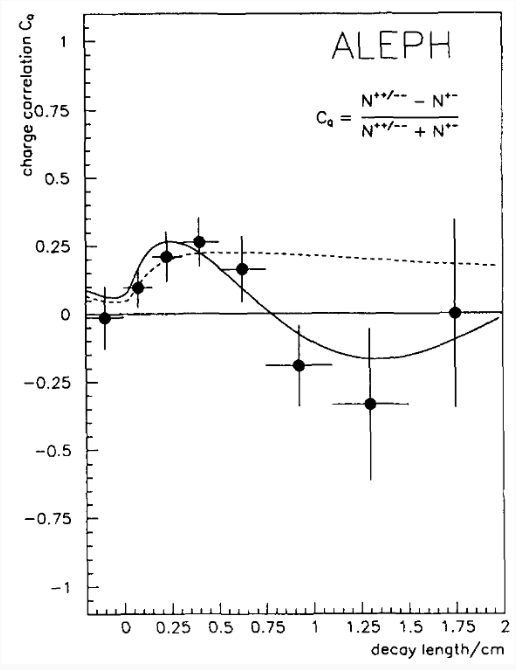
\includegraphics[width=0.3\textwidth]{figs/ALEPHresults.png}
    \caption{Fit to $Q_C(t)$ with a time dependent oscillation in data (solid) and a time independent approach (dashed) \cite{1993498}.}
    \label{fig:ALEPHresults}
\end{wrapfigure}
The ALEPH experiment at LEP measured the oscillation frequency $\upDelta m_d$ by tagging the state of $B_d^0$ at the time of production which decays semileptonic and at the time of decay which decays flavourspecific via $B_d^0\rightarrow D^{*-}X$ and $\bar B_d^0\rightarrow D^{*+}X$ \cite{1993498}.
Every \textit{correct} sign in the decay was defined as an unmixed event and vice versa by which a charge correlation function $C_Q(t)$ was defined.
At ALEPH the $B_d^0$ momentum was not reconstructed and the decay time was not calculated and only the decay length was used with boosting of $B_d^0$ that involved the momentum spectra.
Figure \ref{fig:ALEPHresults} shows an unbinned maximum likelihood fit to the decay length distribution to get $C_Q(t)$.
The involvement of the decay length distribution with the momentum spectra yielded the decay time.
An oscillation frequency of $\upDelta m_d = 0.52^{+0.10}_{-0.11}(\text{stat})^{+0.04}_{-0.05}(\text{syst})\, \text{ps}^{-1}$ was found \cite{1993498}.

\begin{wrapfigure}{l}{6.7cm}
    \centering
    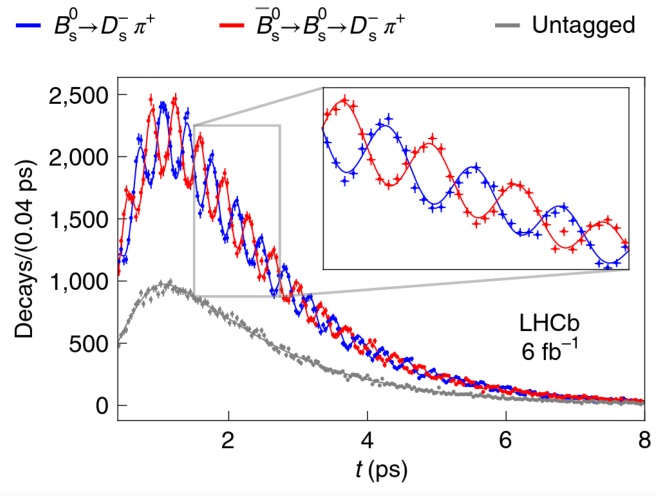
\includegraphics[width=0.48\textwidth]{figs/LHCbResults.png}
    \caption{Measurement of $B_s^0$ oscillations with the LHCb experiment \cite{LHCb2}.}
    \label{fig:LHCbResults}
\end{wrapfigure}
The oscillation of $B_s^0$ is more likely than the $B_d^0$ oscillation, due to $|V_{ts}|>|V_{td}|$ and was first discovered at CDF II in 2006 \cite{PhysRevLett.97.242003}.
Due to the mass difference of $s$ quarks being larger than those of $d$ quarks, a better time resolution was needed.
Measurements of $\upDelta m_d$ with the LHCb experiment at the LHC could increase the precision in 2016 \cite{LHCb1} to a value of $\upDelta m_d = 0.505\pm0.0021\,(\text{stat})\pm0.001\,(\text{syst})\,\text{ps}^{-1}$ leading to a matrix element of $V_{td}=\num{8.6(0.2)e-3}$ \cite{Workman:2022ynf}.
A study from 2022 found an oscillation frequency for $B_s^0$ of $\upDelta m_s = 17.7683 \pm 0.0051\,(\text{stat}) \pm 0.0032\,(\text{syst})\,\text{ps}^{-1}$ \cite{LHCb2} which lead to a value for the matrix element of $V_{ts}=\num{41.5(0.9)e-3}$ \cite{Workman:2022ynf}.
In figure \ref{fig:LHCbResults} the measurements of $B_s^0$ oscillations from the LHCb experiment are shown.
Figure \ref{fig:LHCbResults} shows the decay time of the $B_s^0\rightarrow D_s^-\pi^+$ signal decays are shown with the unmixed components shown in blue and the mixed components shown in red.

% \appendix
% Hier beginnt der Anhang, nummeriert in lateinischen Buchstaben
% \chapter{Appendix}
\label{cha:appendix}

\section{Data Exploration}
\label{sec:DataExploration}

% \begin{figure}[H]
%     \centering
%     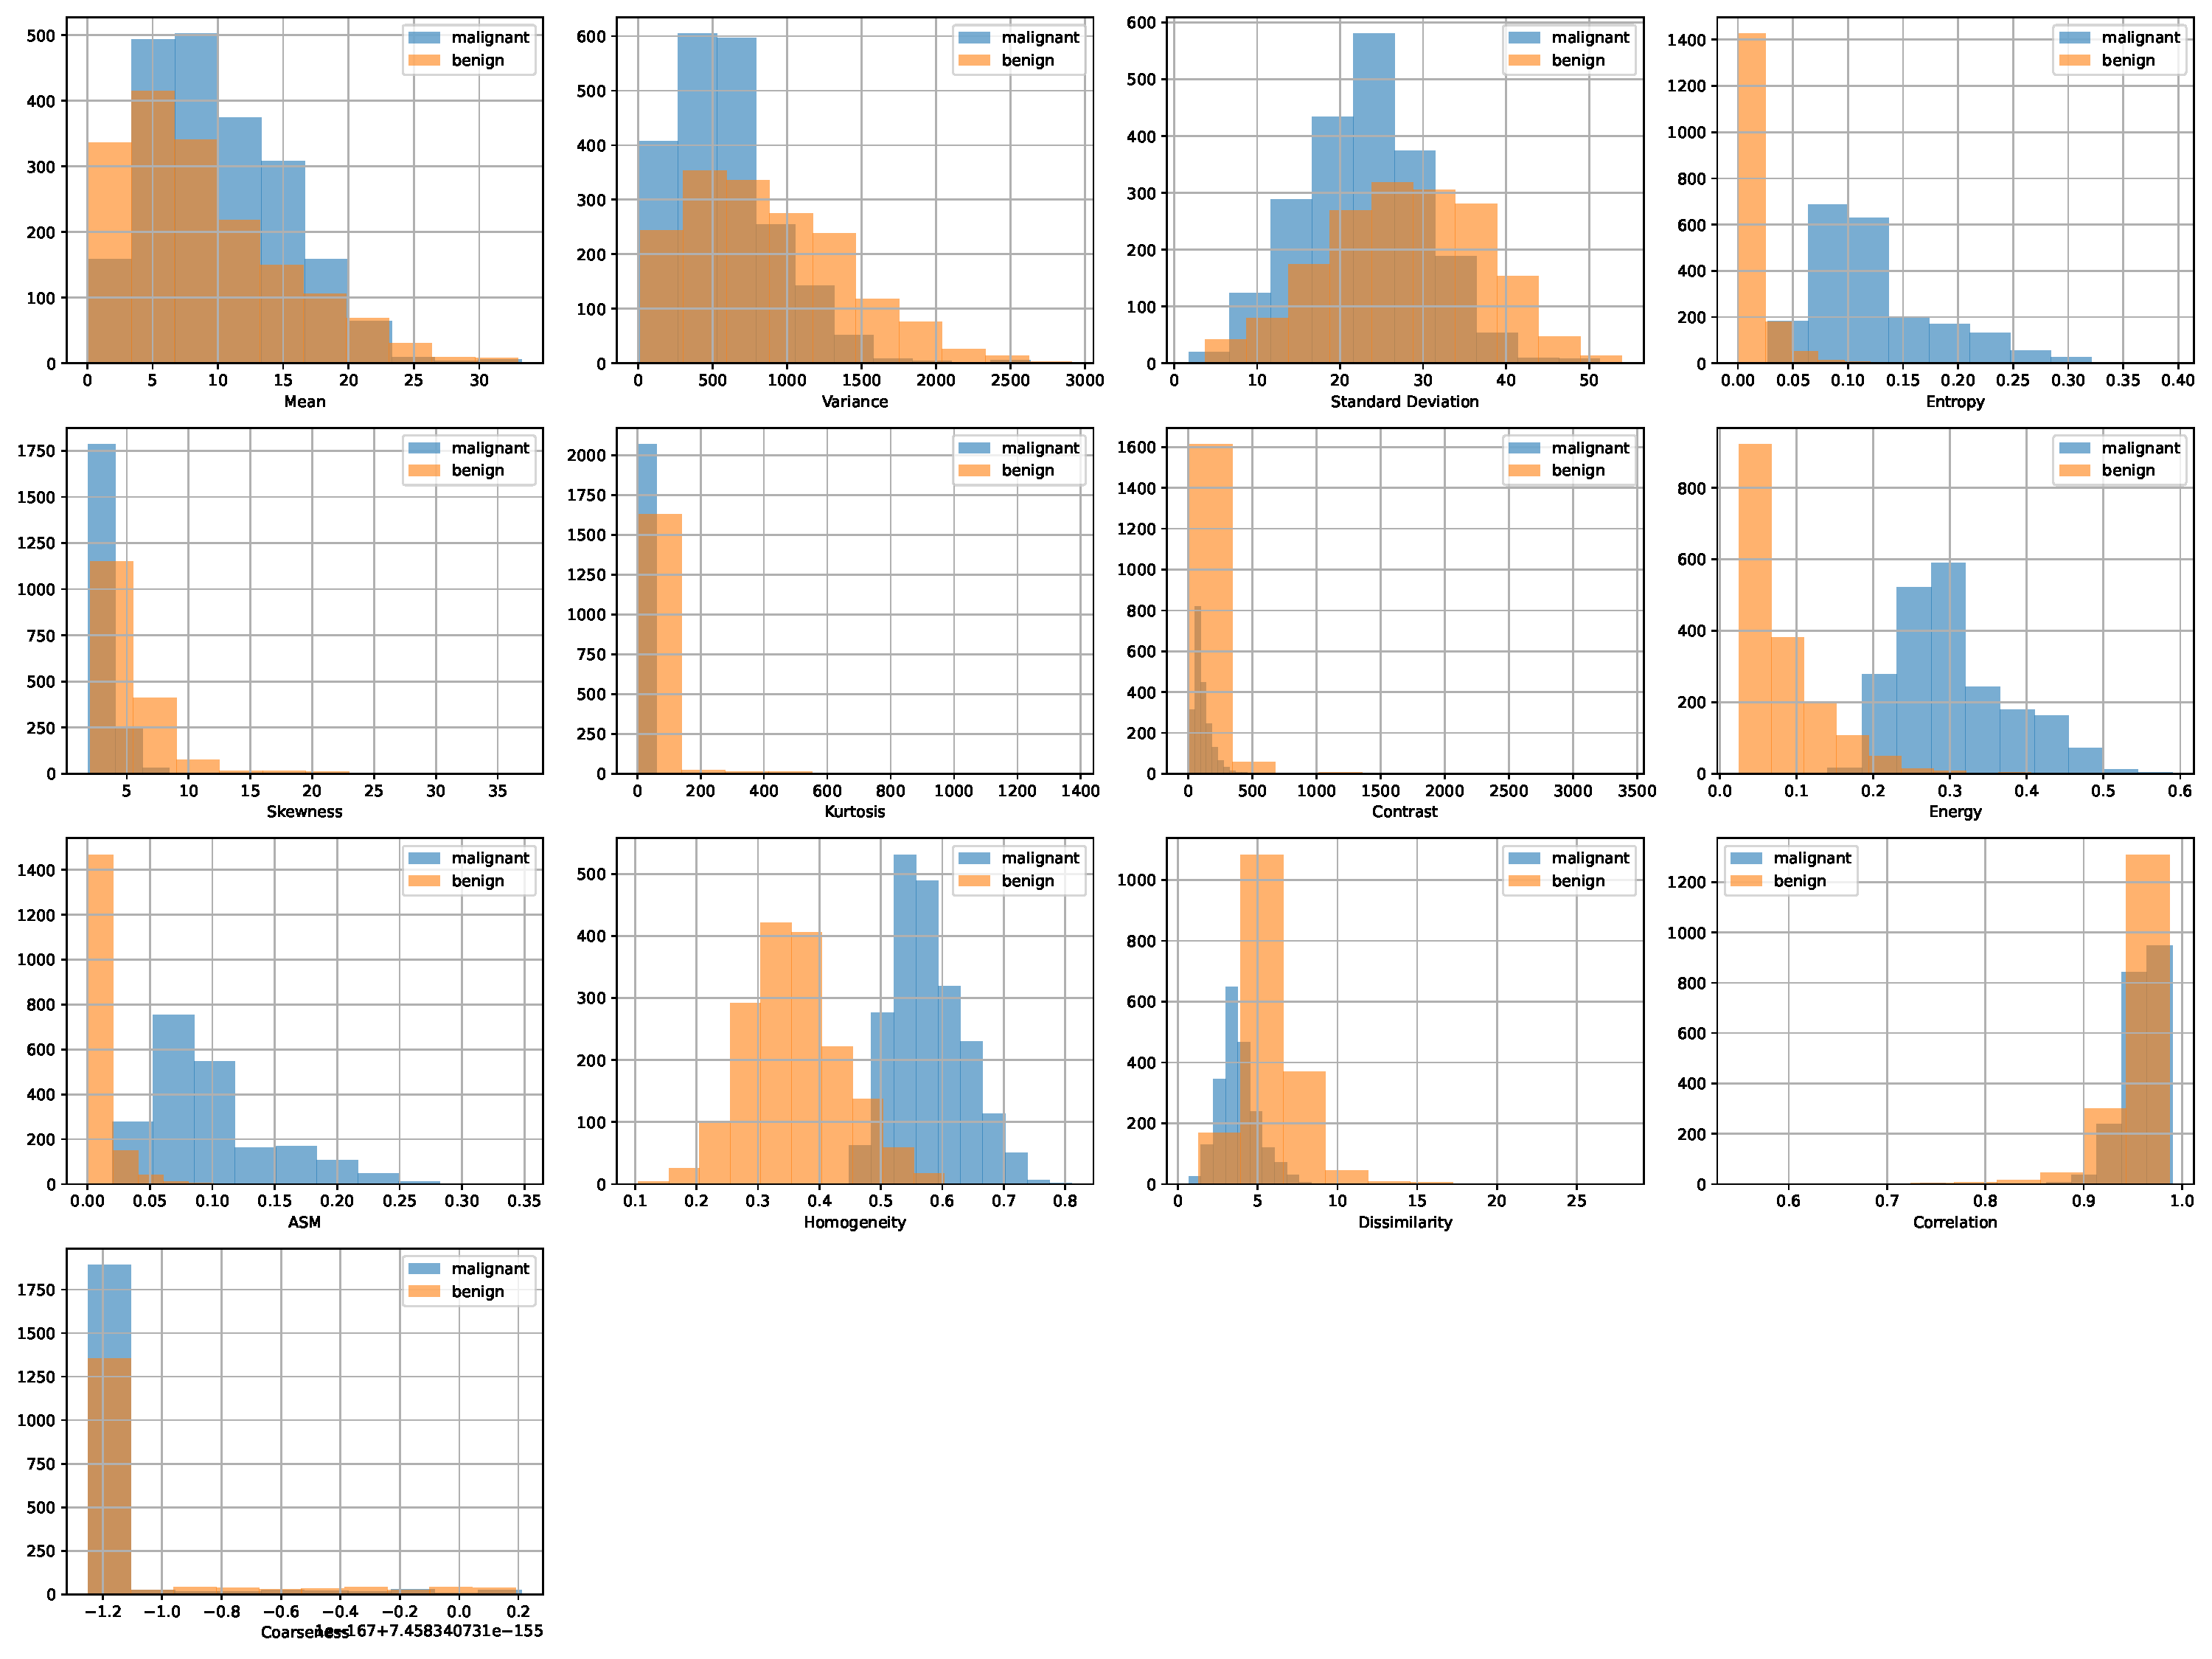
\includegraphics[width=.8\textwidth]{plots/benign_malignant_comparison.pdf}
%     \caption{Comparison between benign and malignant brain tumours for the first- and second-order features.}
%     \label{fig:benign_malignant_comparison}
% \end{figure}

The correlation and scatter matrix of the first- and second-order features are shown in figures \ref{fig:correlation} and \ref{fig:scatter_matrix} respectively.

\begin{figure}[H]
    \centering
    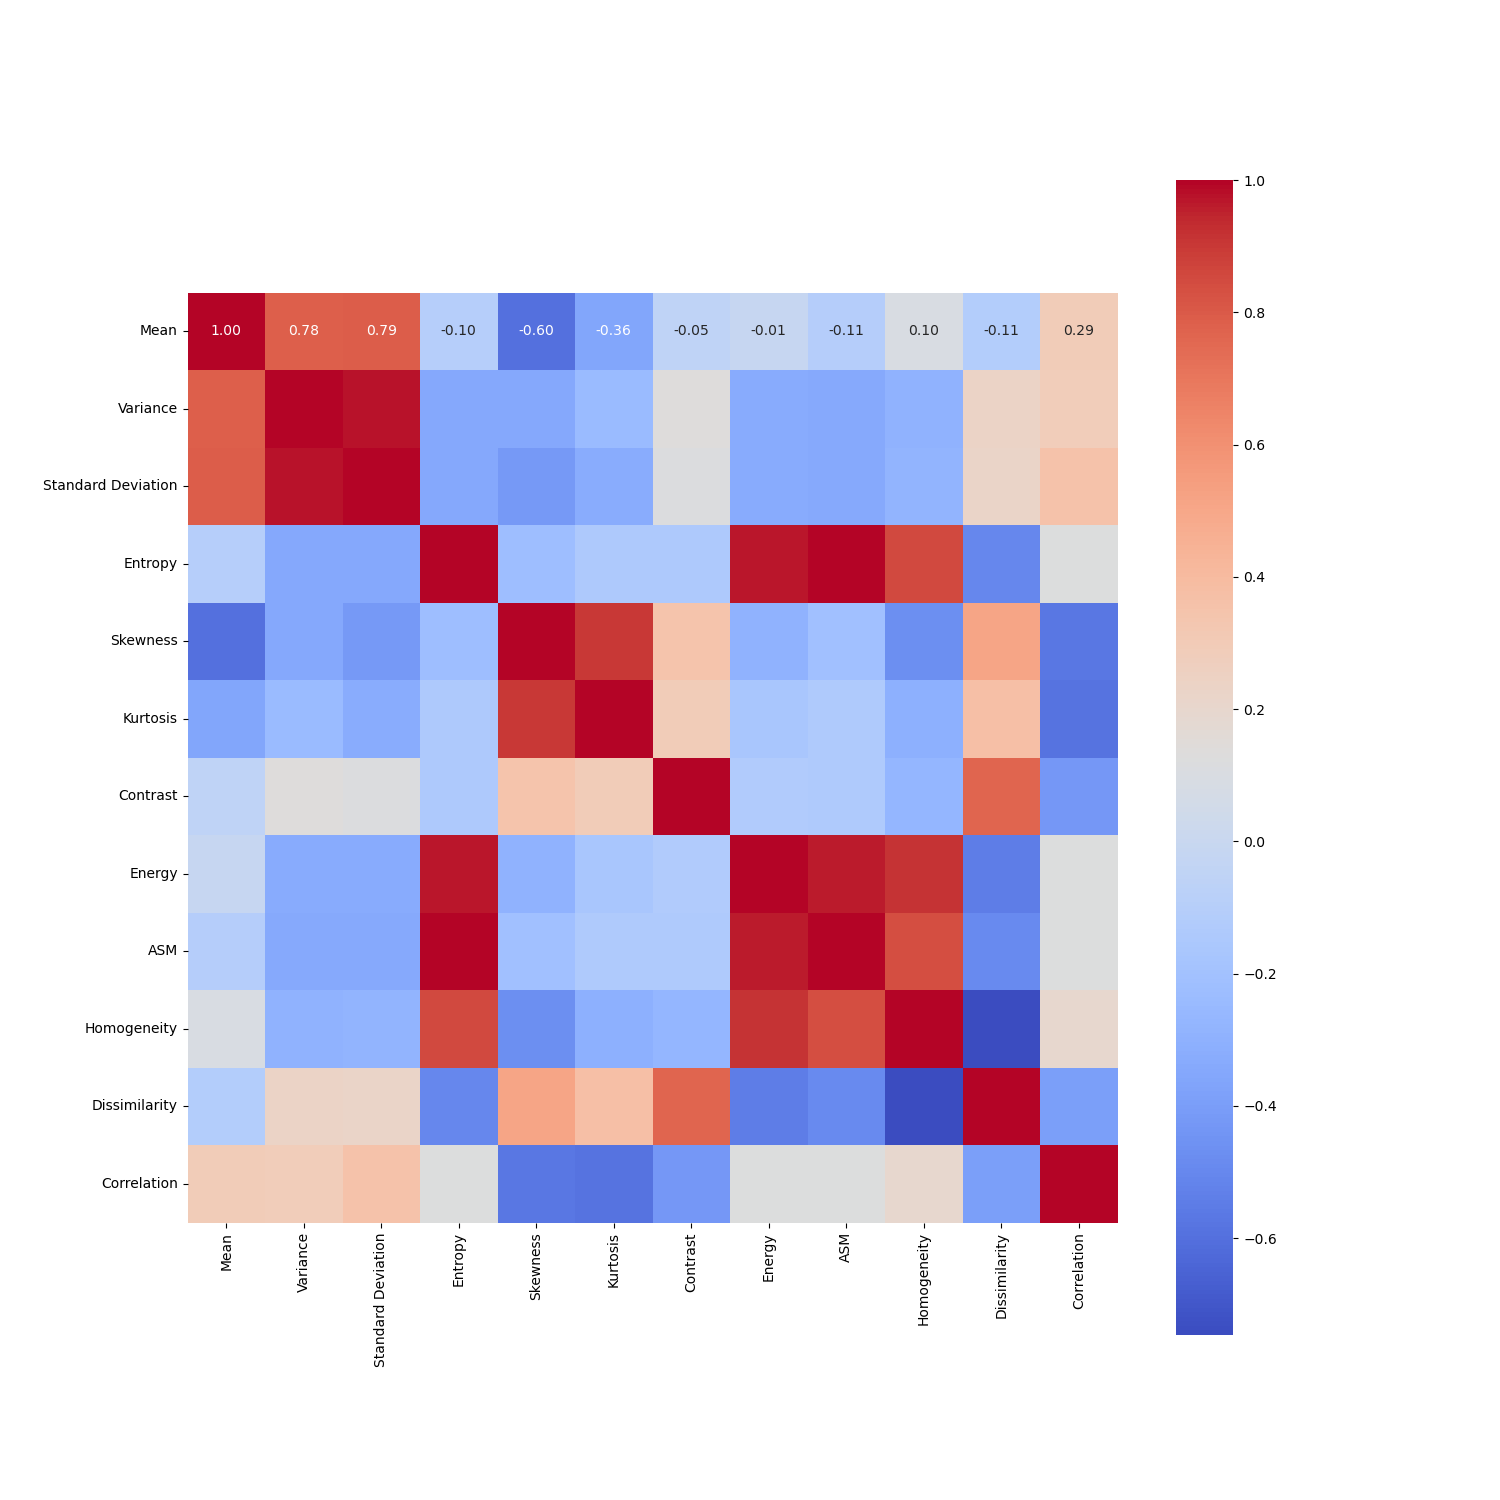
\includegraphics[width=.8\textwidth]{plots/correlation.png}
    \caption{Correlation of the first- and second-order features.}
    \label{fig:correlation}
\end{figure}

\begin{figure}[H]
    \centering
    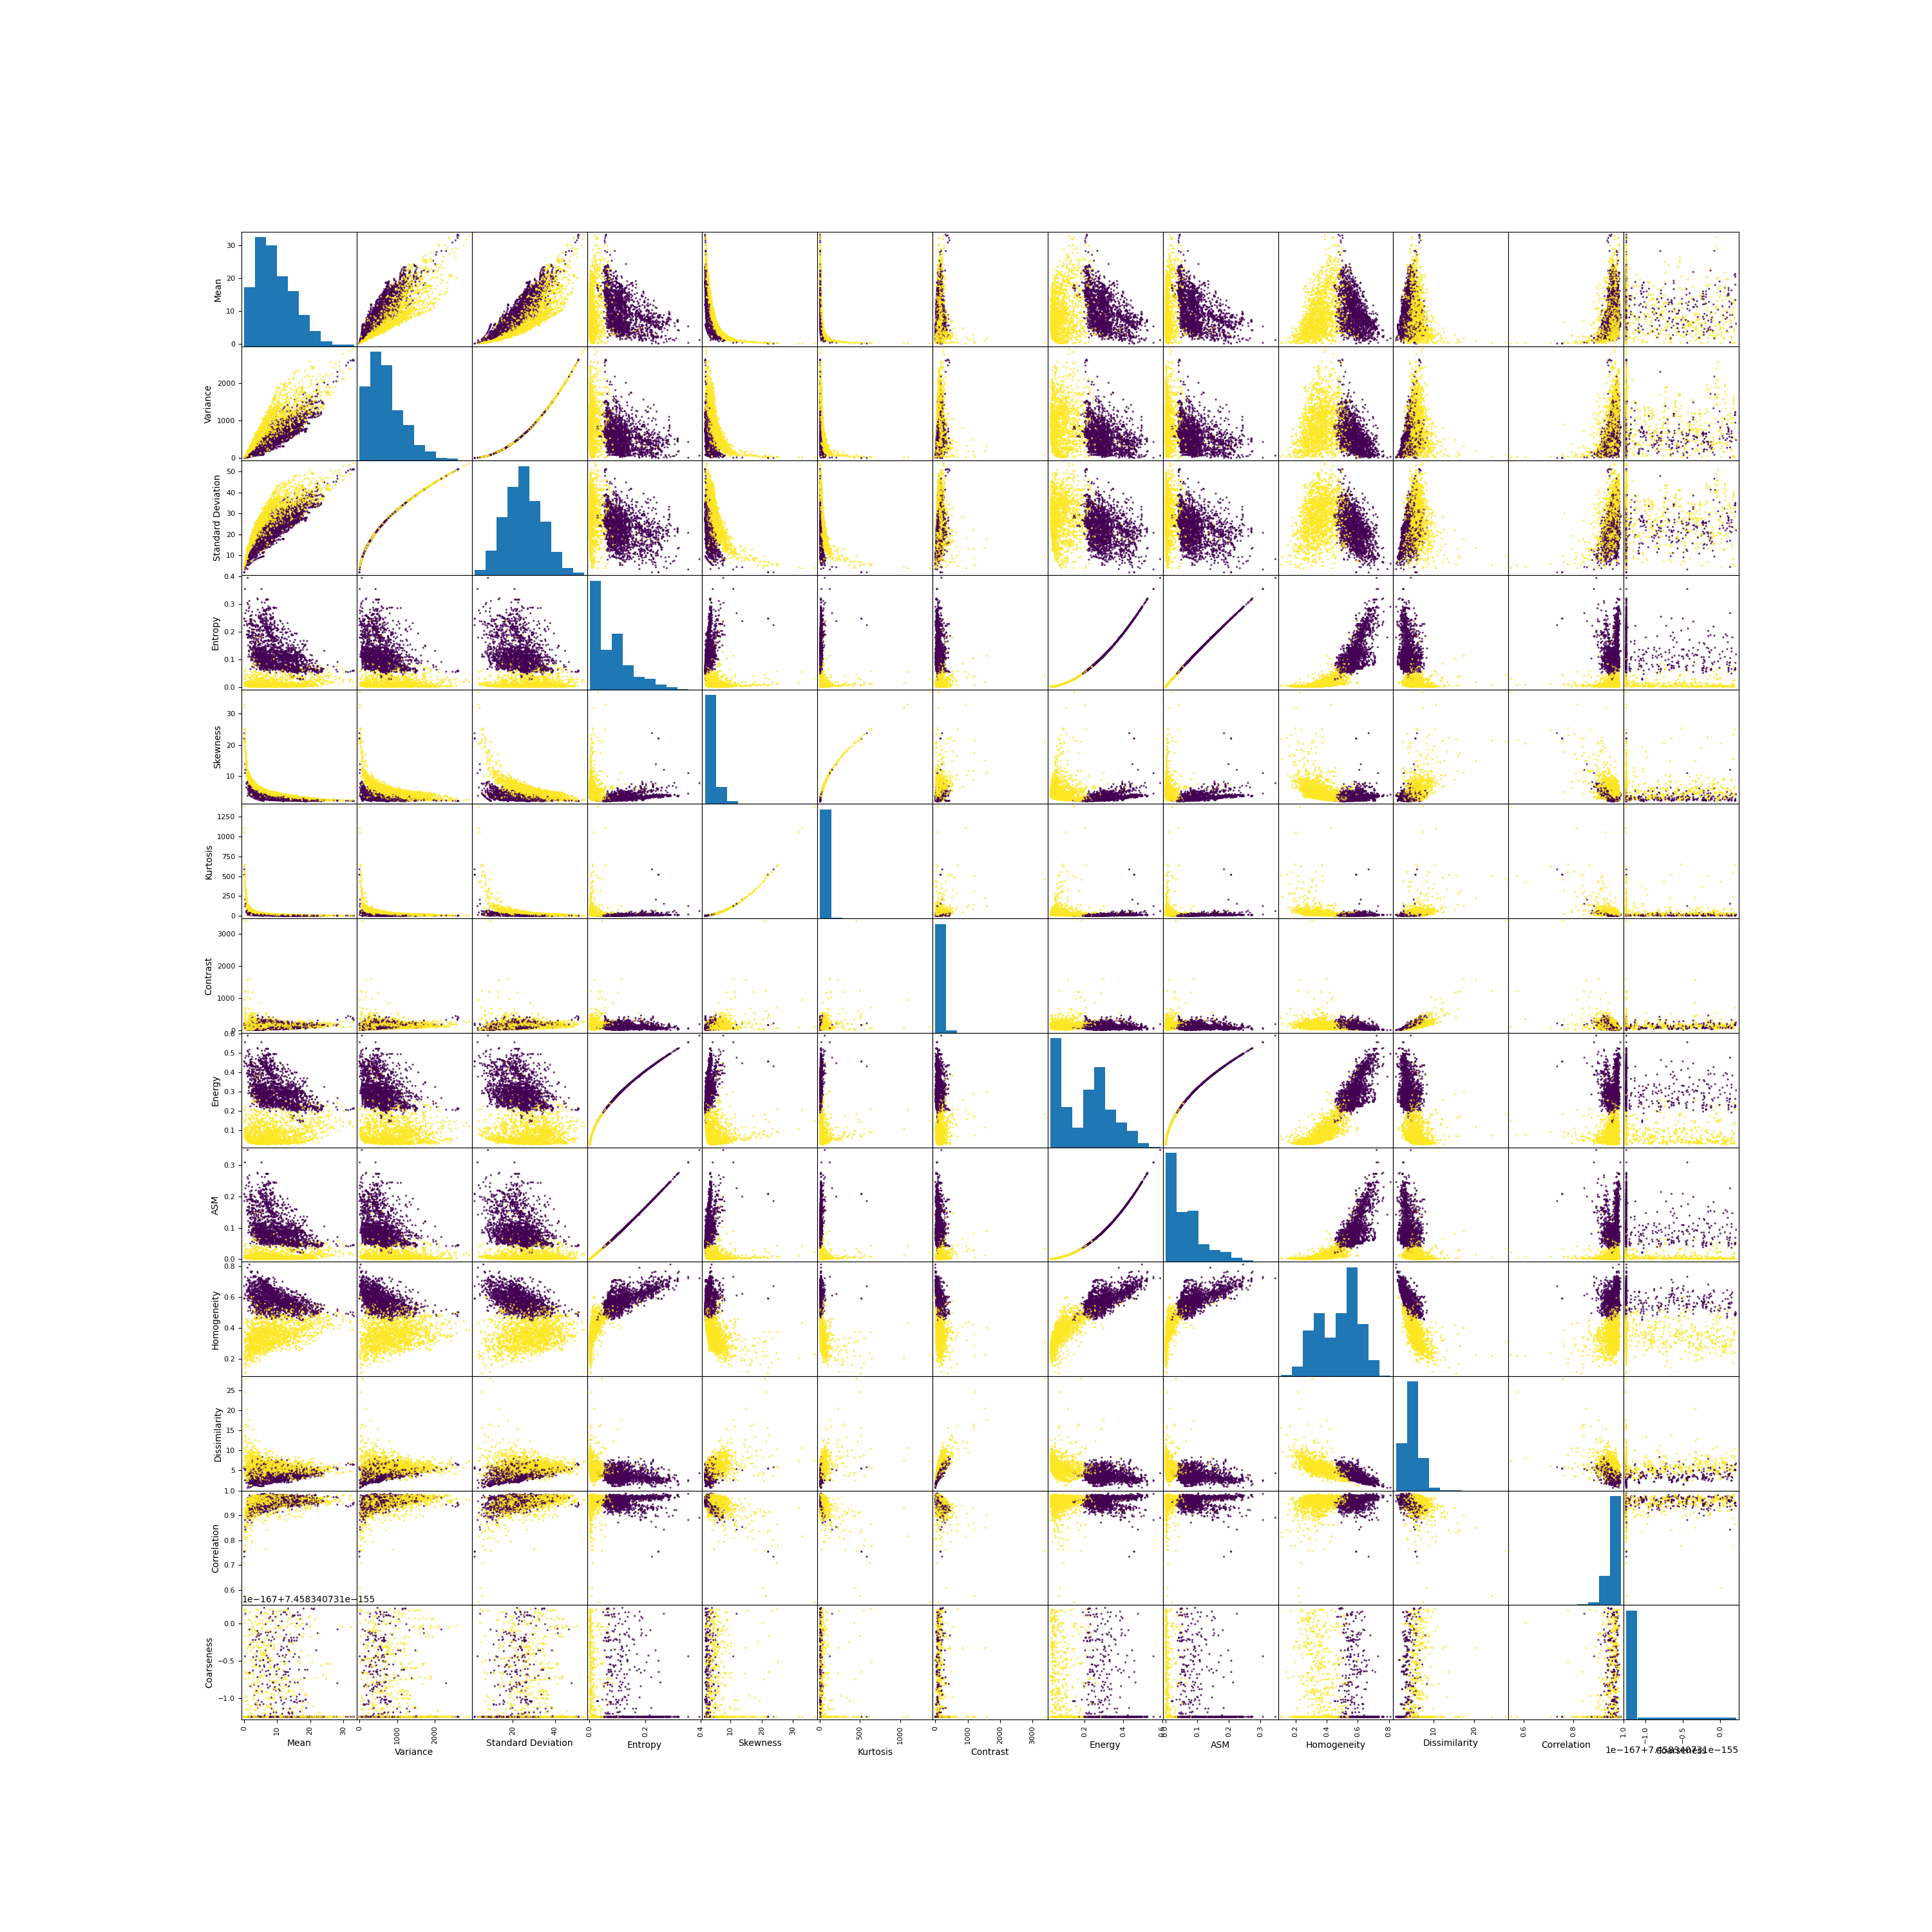
\includegraphics[width=.8\textwidth]{plots/scatter_matrix.png}
    \caption{Scatter matrix of the first- and second-order features.}
    \label{fig:scatter_matrix}
\end{figure}


\section{First Gridsearch Hyperparameter Tests}
\label{sec:FirstGridsearchHyperparameterTests}

Figure \ref{fig:FirstHyperparameterTests} shows the first hyperparameter tests using gridsearch.
This hyperparameter test led to the test, which is described in section \ref{sec:hyperparameter}.
The main goal was to reduce the overfitting, which is why the delta between the training and validation loss was used as the main metric. 
Because the dropout rate decreased the delta between the training and validation loss so much, it was decided to increase the dropout range to 0.6 in the next test.
Because the number of dense units did not have an impact on the delta, a higher range was chosen for the next test.
The range of the number of filters in the convolutional layers was not increased as the delta increased with the number of filters.
There was only taken more data for the next test by using more filters in the same range.

\begin{figure}[H]
    \centering
    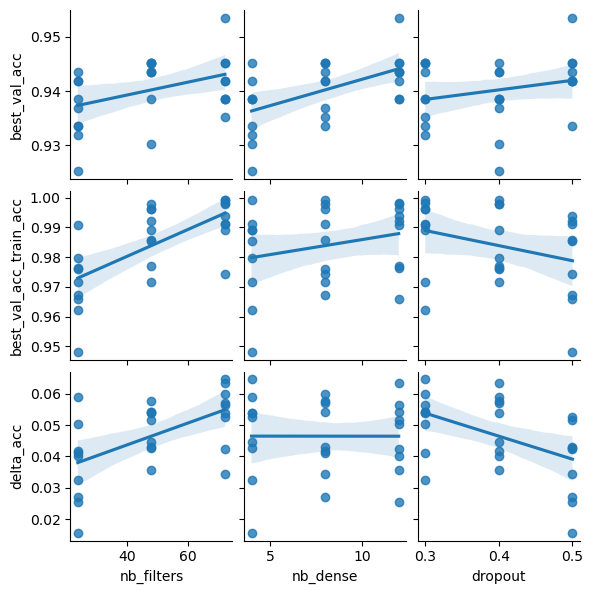
\includegraphics[width=.8\textwidth]{plots/FirstHyperparameterTests.png}
    \caption{First hyperparameter tests using gridsearch.}
    \label{fig:FirstHyperparameterTests}
\end{figure}


\backmatter
\printbibliography

% \cleardoublepage

\end{document}
